\begin{dang}{Đường tiệm cận liên quan tham số $m$}
\end{dang}
\begin{vd}
    Tìm $m$ để đồ thị hàm số
    \begin{listEX}[2]
        \item $y=\dfrac{x-2}{x^2-mx+1}$ có hai đường tiệm cận đứng.
        \item $y=\dfrac{x-1}{x^2-mx+1}$ có đúng ba đường tiệm cận.
        \item $y=\dfrac{\sqrt{x-3}}{x^2+x-m}$ có đúng hai đường tiệm cận.
        \item $y=\dfrac{\sqrt{1-x}}{x^2+4x+m}$ có ba đường tiệm cận.
        %	\item* $y=\dfrac{x}{x^2-2(m+1)x+m^2}$ có đúng hai đường tiệm cận.
    \end{listEX}
    \loigiai{}
\end{vd}
\BTTN
\Opensolutionfile{ans}[ans/2D1-4-DANG-2]
\begin{ex}%[Phạm Văn Long]%[Latex-HK2-TT-2020-2021]%[2D1K4-2]%
    Tìm $m$ để đồ thị hàm số $y=\dfrac{2x^2-3x+4}{x^2+mx+1}$ có duy nhất một đường tiệm cận?
    \choice
    {\True $m\in (-2;2)$}
    {$m\in [-2;2]$}
    {$m\in \{-2;2\}$}
    {$m\in (2;+\infty)$}
    \loigiai{
        Ta thấy đồ thị hàm số đã cho luôn có một tiệm cận ngang là đường $y=2$.\\
        Do đó, để đồ thị hàm số đã cho có duy nhất một đường tiệm cận thì đồ thị hàm số đã cho không có tiệm cận đứng.\\
        $\Rightarrow$ Phương trình $x^2+mx+1=0$ vô nghiệm $\Leftrightarrow \Delta <0 \Leftrightarrow m^2-4<0\Leftrightarrow m\in (-2;2)$.
    }
\end{ex}
\begin{ex}%[2D1K4-2]%[Đề GHK1, THPT Trần Nhân Tông, Hà Nội 2018]%[WTT2D1-128]%
    Tìm giá trị thực của tham số $m$ để đồ thị hàm số $y=\dfrac{x-4}{m-x^2}$ có đường tiệm cận đứng.
    \choice
    {$m\ge0;\,m\ne16$}
    {\True $m\ge0$}
    {$m>0$}
    {$m>0;\,m\ne16$}
    \loigiai{
        Điều kiện xác định: $m-x^2\neq0$.\\
        Để đồ thị hàm số có đường tiệm cận đứng thì phương trình $m-x^2=0$ có nghiệm, tức là $m\ge0$.\\
        Với $m=16$ thì $y=\dfrac{-1}{4+x}$ có một tiệm cận đứng là $x=-4$. Vậy giá trị $m$ cần tìm là $m\ge0$.
    }
\end{ex}
\begin{ex}%[2D1K4-2]%
    Có bao nhiêu giá trị của tham số $m$ thoả mãn đồ thị hàm số $y=\dfrac{x+3}{x^2-x-m}$ có đúng hai đường tiệm cận?
    \choice
    {$1$}
    {$4$}
    {\True $2$}
    {$3$}
    \loigiai{
        Đồ thị hàm số có đúng hai đường tiệm cận khi phương trình $x^2-x-m=0$ có nghiệm kép hoặc có hai nghiệm phân biệt với một nghiệm bằng $-3$. Khi đó
        \[\hoac{&\Delta=0\\&\heva{&\Delta>0\\&g(-3)=0}}\Leftrightarrow\hoac{&4m+1=0\\&\heva{&4m+1>0\\&m=12}}\hoac{&m=-\dfrac{1}{4}\\&m=12.}\]
        Vậy có hai giá trị của m.}
\end{ex}
\begin{ex}%[2D1K4-2]%[Đề kiểm tra giữa học kì I, 2017 - 2018 trường THPT Chu Văn An, Hà Nội]%[WTT2D1-156]%
    Tìm tất cả các giá trị thưc của tham số $m$ để đồ thị hàm số $y=\dfrac{x^2+m}{x^2-3x+2}$ có đúng hai tiệm cận.
    \choice
    {$m=-1$}
    {$m\in\left\{1;4\right\}$}
    {\True $m\in\left\{-1;-4\right\}$}
    {$m=4$}
    \loigiai{
        Vì $\lim\limits_{x\to\pm\infty}\dfrac{x^2+m}{x^2-3x+2}=1,\,\forall m$ nên đồ thị hàm số luôn có một tiêm cận ngang là $y=1$.\\
        Để đồ thị hàm số có đúng hai tiệm cận thì đồ thị hàm số có thêm một tiệm cận đứng là $x=1$ hoặc là $x=2$.
        \begin{itemize}
            \item Đồ thị hàm số có một tiệm cận đứng $x=1$, suy ra pt $x^2+m=0$ và phương trình $x^2-3x+2=0$ có nghiệm chung là $x=1\Rightarrow m=-1$.
            \item Đồ thị hàm số có một tiệm cận đứng $x=2$, suy ra pt $x^2+m=0$ và phương trình $x^2-3x+2=0$ có nghiệm chung là $x=2\Rightarrow m=-4$.
        \end{itemize}
        Vậy $m\in\left\{-1;4\right\}$ thỏa yêu cầu bài toán.
    }
\end{ex}
\begin{ex}%[Thi thử, THPT Lục Ngạn - Bắc Giang, 2019]%[Trần Như Ngọc, 12EX3-2019]%[2D1K4-2]%
    Có bao nhiêu giá trị nguyên dương của tham số $m$ để đồ thị hàm số
    $y=\dfrac{\sqrt{9-x}}{x^2-2(m+1)x+m^2+2m}$
    có đúng hai đường tiệm cận.
    \choice
    {\True $2$}
    {$1$}
    {$4$}
    {$3$}
    \loigiai{
        Ta có $ x^2-2(m+1)x+m^2+2m = 0 \Leftrightarrow \hoac{& x=m \\ & x=m+2}$
        $( \Delta ' = 1 )$. \\
        Hàm số xác định khi $ \heva{& x \le 9 \\ & x \ne m \\ & x \ne m+2.} $\\
        Ta có $\lim \limits_{x\to -\infty}y = 0$ nên đồ thị hàm số có một tiệm cận ngang là $ y = 0 $.\\
        Đồ thị hàm số có đúng hai tiệm cận khi và chỉ khi nó có đúng một tiệm cận đứng \\
        $\Leftrightarrow$ phương trình trên có một nghiệm nhỏ hơn hoặc bằng $ 9 $.\\
        $\Leftrightarrow m \le 9 < m+2 \Leftrightarrow 7 < m \le 9 $.\\
        Vậy có $ 2 $ giá trị $ m $ nguyên dương thỏa mãn điều kiện bài toán.
    }
\end{ex}
\begin{ex}%[Thi học kỳ I, Trường THPT Chuyên Lê Quý Đôn - Khánh Hòa, 2021]%[Lê Hồng Phi, 12EX5]%[2D1K4-2]%
    Cho hàm số $y=\dfrac{2x-3}{\sqrt{x^2+2(m-2)x+m^2}}$ với $m$ là tham số thực và $m>1$. Hỏi đồ thị hàm số có bao nhiêu đường tiệm cận (tiệm cận ngang và tiệm cận đứng)?
    \choice
    {$1$}
    {\True $2$}
    {$3$}
    {$4$}
    \loigiai
    {Phương trình $x^2+2(m-2)x+m^2=0$ có $\Delta'=(m-2)^2-m^2=-2(2m-2)=-4(m-1)<0,\ \forall m>1$ nên vô nghiệm.\\
        Do đó tập xác định của hàm số là $\mathscr{D}=\mathbb{R}$.\\
        Như thế đồ thị hàm số không có đường tiệm cận đứng.\\
        Ta tính được
        \begin{itemize}
            \item $\lim\limits_{x\to +\infty}y=\lim\limits_{x\to +\infty}\dfrac{2-\dfrac{3}{x}}{\sqrt{1+\dfrac{2(m-2)}{x}+\dfrac{m^2}{x}}}=2$ nên $y=2$ là đường tiệm cận ngang.
            \item $\lim\limits_{x\to -\infty}y=\lim\limits_{x\to -\infty}\dfrac{2-\dfrac{3}{x}}{-\sqrt{1+\dfrac{2(m-2)}{x}+\dfrac{m^2}{x}}}=-2$ nên $y=-2$ là đường tiệm cận ngang.
        \end{itemize}
        Vậy đồ thị hàm số đã cho có $2$ đường tiệm cận.
    }
\end{ex}
\begin{ex}%[Đề Khảo sát lần 1 THPT Quang Hà - Vĩnh Phúc, 2021]%[Trần Nhân Kiệt, 12EX4-2021]%[2D1K4-2]%
    Có bao nhiêu giá trị nguyên của tham số $m$ để đồ thị tham số $y=\dfrac{1+\sqrt{x+1}}{\sqrt{x^2-(1-m)x+2m}}$ có hai tiệm cận đứng?
    \choice
    {$2$}
    {\True $3$}
    {$1$}
    {$0$}
    \loigiai{
        Điều kiện $\heva{& x\ge -1 \\ & x^2-(1-m)x+2m>0.}$\\
        Đồ thị hàm số có hai tiệm cận đứng khi và chỉ khi phương trình $x^2-(1-m)x+2m=0$ có hai nghiệm phân biệt lớn hơn hoặc bằng $-1$.\\
        Ta có $x^2-(1-m)x+2m=0\Leftrightarrow x^2-x+m(x+2)=0\Leftrightarrow m=\dfrac{-x^2+x}{x+2}$.\\
        Đặt $f(x)=\dfrac{-x^2+x}{x+2}$, $x\ge -1$.\\
        Ta có $f'(x)=\dfrac{-x^2-4x+2}{(x+2)^2}$, suy ra $f'(x)=0\Leftrightarrow -x^2-4x+2=0\Leftrightarrow x=-2\pm \sqrt{6}$.
        \begin{center}
            \begin{tikzpicture}[>=stealth]
                \tkzTabInit[nocadre=false,lgt=1.2,espcl=3,deltacl=0.5]
                {$x$/.7 ,$f'(x)$/.7,$f(x)$/2}
                {$-1$ , $-2+\sqrt{6}$ , $+\infty$}
                \tkzTabLine{ , - , $0$ , + , }
                \tkzTabVar{-/$-2$ , +/$5-2\sqrt{6}$ , -/$-\infty$}
            \end{tikzpicture}
        \end{center}
        Từ bảng biến thiên suy ra $m\in [-2;5-2\sqrt{6})$.\\
        Vì $m$ nguyên nên $m\in \{-2;-1;0\}$.\\
        Vậy có $3$ giá trị nguyên của $m$ thỏa mãn bài.
    }
\end{ex}
\BTTL
\begin{ex}%[2D1K4-2]%
    Cho hàm số $y=\dfrac{2x^2-3x+m}{x-m}$ có đồ thị $(C)$. Với tất cả các giá trị thực nào của tham số $m$ thì đồ thị $(C)$ không có tiệm cận đứng?
    \shortans{$m=0$ hoặc $m=1$}
    %	\choice
    %	{$m=2$}
    %	{$m=0$}
    %	{$m=1$}
    %	{\True $m=0$ hoặc $m=1$}
    \loigiai{
        Đồ thị không có tiệm cận đứng khi $x=m$ là nghiệm của phương trình $2x^2-3x+m=0$, suy ra $2m^2-3m+m=0 \Leftrightarrow \hoac{&m=0\\&m=1}$.
    }
\end{ex}
\begin{ex}%[2D1K4-2]%
    Với tất cả các giá trị thực nào của tham số $m$ thì đồ thị hàm số $y=\dfrac{x^2+x-2}{x^2+x+m}$ có ba đường tiệm cận?
    \shortans{$m<\dfrac{1}{4}$ và $m\ne -2$}
    %	\choice
    %	{$m>\dfrac{1}{4}$ và $m\ne 2$}
    %	{$m>\dfrac{1}{4}$}
    %	{$m<\dfrac{1}{4}$}
    %	{\True $m<\dfrac{1}{4}$ và $m\ne -2$}
    \loigiai{
        Đồ thị hàm số chỉ có $1$ tiệm cận ngang là $y=1$.\\
        Ta có $x^2+x-2 \Leftrightarrow \hoac{&x=1\\&x=-2.}$\\
        Đồ thị hàm số có ba đường tiệm cận khi và chỉ khi có $2$ tiệm cận đứng. Điều này tương đương với phương trình $x^2+x+m=0$ có $2$ nghiệm phân biệt khác $1$ và $-2$, nghĩa là\\
        $\heva{&1-4m>0\\&1^2+1+m \ne 0\\& (-2)^2-2+m\ne 0} \Leftrightarrow \heva{&m<\dfrac{1}{4}\\&m\ne -2.}$
    }
\end{ex}
\begin{ex}%[đề thi thử THPT Quốc gia, đề số 3, nguyễn hoàng thanh]%[2D1K4-2]%
    Tìm số giá trị nguyên thuộc đoạn $ [-2025;2025] $ của tham số $ m $ để đồ thị hàm số $ y=\dfrac{\sqrt{x-3}}{x^2+x-m} $ có đúng hai đường tiệm cận.
    \shortans{$2014$}
    %	\choice
    %	{$ 2007 $}
    %	{$ 2010 $}
    %	{$ 2009 $}
    %	{\True $ 2008 $}
    \loigiai{
        Điều kiện xác định của hàm số $ \heva{& x\ge 3\\& x^2+x-m\ne 0.} $\\
        Vì $ \lim\limits_{x\to +\infty}\dfrac{\sqrt{x-3}}{x^2+x-m}=\lim\limits_{x\to +\infty}\dfrac{\sqrt{\frac{1}{x}-\frac{3}{x^2 }}}{1+\frac{1}{x}-\frac{m}{x^2}}=0 $, suy ra $ y=0 $ là tiệm cận ngang.\\
        Để đồ thị hàm số có đúng hai tiệm cận thì đồ thị hàm số chỉ có thêm một tiệm cận đứng, tương đương $ f(x)=x^2+x-m $ có đúng một nghiệm lớn hơn $ 3 $. Xét các trường hợp xảy ra như sau
        \begin{enumerate}
            \item $ f(x)=0 $ có nghiệm kép $ x_{1}=x_2=-\dfrac{1}{2}<3 $ (không thỏa mãn).
            \item $ f(x)=0 $ có hai nghiệm thỏa $ x_1<3\le x_2\Leftrightarrow a\cdot f(3)\le 0\Leftrightarrow 12-m\le 0\Leftrightarrow m\ge 12 $.
        \end{enumerate}
        Kết hợp với yêu cầu bài toán ta suy ra $ \heva{&m\in \mathbb{Z}\\ &m\in[12;2025]} $, suy ra có $ 2025-12+1=2014 $ giá trị nguyên của $ m $ thỏa mãn bài toán.
    }
\end{ex}
\begin{ex}%[Đề tham khảo THPT Quốc gia 2021 - Đề 5]%[Đoàn Minh Tân]%[2D1K4-2]%
    Tìm tất cả giá trị thực của tham số $m$ để đồ thị hàm số $y=\dfrac{3x+2018}{\sqrt{mx^2+5x+6}}$ có hai đường tiệm cận ngang.
    \shortans{$m>0$}
    %	\choice
    %	{$m\in \varnothing$}
    %	{$m<0$}
    %	{$m=0$}
    %	{\True $m>0$}
    \loigiai{
        Ta có $\displaystyle \lim \limits_{x\to +\infty} y=\displaystyle\lim\limits_{x\to +\infty}\dfrac{3x+2018}{\sqrt{mx^2+5x+6}}=\displaystyle\lim\limits_{x\to +\infty}\dfrac{3+\dfrac{2018}{x}}{\sqrt{m+\dfrac{5}{x}+\dfrac{6}{x^2}}}=\dfrac{3}{\sqrt{m}}$ tồn tại khi $m>0$.\\
        $\displaystyle\lim\limits_{x\to -\infty}=\displaystyle\lim\limits_{x\to -\infty}\dfrac{3x+2018}{\sqrt{mx^2+5x+6}}=\displaystyle\lim\limits_{x\to -\infty}\dfrac{3+\dfrac{2018}{x}}{-\sqrt{m+\dfrac{5}{x}+\dfrac{6}{x^2}}}=-\dfrac{3}{\sqrt{m}}$ tồn tại khi $m>0$.\\
        Hiên nhiên $\displaystyle\lim\limits_{x\to +\infty}y\ne \displaystyle \lim \limits_{x\to -\infty}y$.\\
        Vậy đồ thị hàm số đã cho có hai tiệm cận ngang khi và chỉ khi $m>0$.
    }
\end{ex}
\begin{ex}%[2D1K4-2]%
    Có bao nhiêu giá trị nguyên của tham số thực $m$ thuộc đoạn $[-20; 10]$ để đồ thị hàm số $y=\dfrac{x+2}{\sqrt{x^2-4x+m}}$ có hai đường tiệm cận đứng?
    \shortans{$23$}
    %	\choice
    %	{$20$}
    %	{$21$}
    %	{$22$}
    %	{\True $23$}
    \loigiai{
        Đồ thị hàm số có hai đường tiệm cận đứng $\Leftrightarrow$ phương trình $x^2-4x+m=0$ có hai nghiệm phân biệt khác $-2$ \\
        $ \Leftrightarrow\heva{&2^2-m>0\\&(-2)^2-4\cdot (-2)+m\neq 0}\Leftrightarrow\heva{&m<4\\&m\neq-12.} $ \\
        Do $m$ nguyên và $m\in[-20; 10]$ nên $m\in\left\{-20;-19;\ldots;-13;-11;\ldots; 2; 3\right\}$, gồm $23$ giá trị thỏa mãn.}
\end{ex}
\Closesolutionfile{ans}